% This file was created with tikzplotlib v0.10.1.
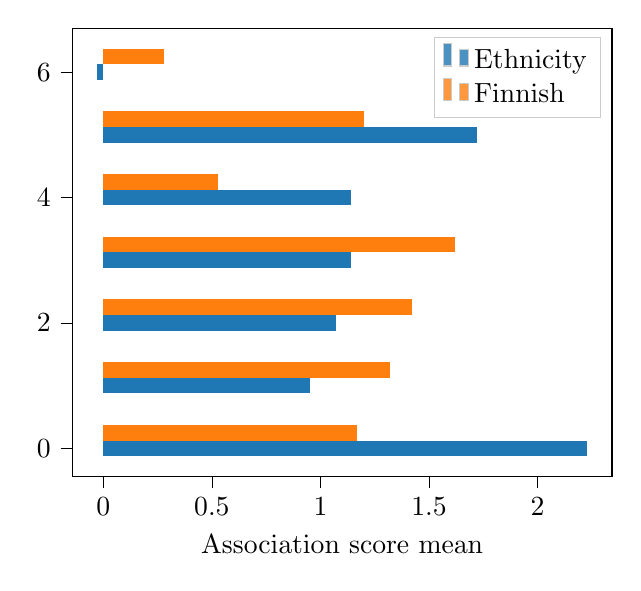
\begin{tikzpicture}

\definecolor{darkgray176}{RGB}{176,176,176}
\definecolor{darkorange25512714}{RGB}{255,127,14}
\definecolor{lightgray204}{RGB}{204,204,204}
\definecolor{steelblue31119180}{RGB}{31,119,180}

\begin{axis}[
legend cell align={left},
legend style={fill opacity=0.8, draw opacity=1, text opacity=1, draw=lightgray204},
tick align=outside,
tick pos=left,
x grid style={darkgray176},
xlabel={Association score mean},
xmin=-0.143, xmax=2.343,
xtick style={color=black},
y grid style={darkgray176},
ymin=-0.45, ymax=6.7,
ytick style={color=black}
]
\draw[draw=none,fill=steelblue31119180] (axis cs:0,-0.125) rectangle (axis cs:2.23,0.125);
\addlegendimage{ybar,ybar legend,draw=none,fill=steelblue31119180}
\addlegendentry{Ethnicity}

\draw[draw=none,fill=steelblue31119180] (axis cs:0,0.875) rectangle (axis cs:0.95,1.125);
\draw[draw=none,fill=steelblue31119180] (axis cs:0,1.875) rectangle (axis cs:1.07,2.125);
\draw[draw=none,fill=steelblue31119180] (axis cs:0,2.875) rectangle (axis cs:1.14,3.125);
\draw[draw=none,fill=steelblue31119180] (axis cs:0,3.875) rectangle (axis cs:1.14,4.125);
\draw[draw=none,fill=steelblue31119180] (axis cs:0,4.875) rectangle (axis cs:1.72,5.125);
\draw[draw=none,fill=steelblue31119180] (axis cs:0,5.875) rectangle (axis cs:-0.03,6.125);
\draw[draw=none,fill=darkorange25512714] (axis cs:0,0.125) rectangle (axis cs:1.17,0.375);
\addlegendimage{ybar,ybar legend,draw=none,fill=darkorange25512714}
\addlegendentry{Finnish}

\draw[draw=none,fill=darkorange25512714] (axis cs:0,1.125) rectangle (axis cs:1.32,1.375);
\draw[draw=none,fill=darkorange25512714] (axis cs:0,2.125) rectangle (axis cs:1.42,2.375);
\draw[draw=none,fill=darkorange25512714] (axis cs:0,3.125) rectangle (axis cs:1.62,3.375);
\draw[draw=none,fill=darkorange25512714] (axis cs:0,4.125) rectangle (axis cs:0.53,4.375);
\draw[draw=none,fill=darkorange25512714] (axis cs:0,5.125) rectangle (axis cs:1.2,5.375);
\draw[draw=none,fill=darkorange25512714] (axis cs:0,6.125) rectangle (axis cs:0.28,6.375);
\end{axis}

\end{tikzpicture}
